\documentclass[12pt]{article}

% Essential packages
\usepackage[utf8]{inputenc}
\DeclareUnicodeCharacter{2002}{\enspace}
\usepackage[margin=1in]{geometry}
\usepackage[numbers]{natbib}
\usepackage{pgfplots}
\pgfplotsset{compat=1.18}
\usepackage{float}
\usepackage{booktabs}
\usepackage{longtable}
\usepackage{graphicx}
\usepackage{amsmath}
\usepackage{amssymb}
\usepackage[colorlinks=true, linkcolor=blue, urlcolor=blue, citecolor=blue]{hyperref}

% Typography improvements
\usepackage{microtype}
\usepackage{setspace}
\onehalfspacing

% Title formatting
\title{\Large\bfseries Evaluating the Efficacy of Large Language Models for Geolocation Identification}

\author{
  Rohan Poudel
  \and
  Om Goswami
}

\date{}

\begin{document}

\maketitle

\begin{abstract}
Multimodal large language models have shown remarkable performance in image-based geolocation, but so far there is little understanding of how well they generalize to new environments. We assess two modern state-of-the-art models, Gemini 2.5 Pro and GPT-5, on a set of 2,600 varied street-view and community-driven images via Chain-of-Thought prompting. Prior work has found that although state-of-the-art models can attain human-level or even higher quality on competitive GeoLoc tasks, little is known about their error distributions. Our approach is one of systematic evaluation on five levels of geographic precision, ranging from accurate modeling at the street level to large-scale errors spanning continents, as well as examining not only where models succeed but also in which ways they fail. We find that models with the same overall accuracy have decidedly non-uniform error patterns. All predictions by GPT-5 are within 250 km of the region, but this is not clear for Gemini 2.5 Pro where about 30\% of the predictions are in the distance range between 250--1000 km. These gaps have real practical deployment implications: the applications that demand predictable accuracy would rather know entire error distributions and not just blindly trust average performance metrics.
\end{abstract}

\section{Introduction}

Multimodal large language models have shown impressive performance for image-based geolocation by deducing locations from environmental signals, such as architectural styles, patterns of vegetation, or infrastructure \cite{Liu2024,Campos2025}. Recently developed models, such as ETHAN, lead to high performance in competitive geolocation tasks \cite{Liu2024}, and have been applied to analyzing historical documents \cite{Mioduski2025}, assessing privacy risks \cite{Liu2025} and city planning \cite{Feng2025}.

Nevertheless, the current evaluations mainly concentrate on mean accuracy measures, and fail to reveal important behavioral deviations. Average error measurements can give only very partial information about the distribution of errors: two models with the same mean performance may be making very different mistakes. Knowledge of these behavioral profiles is just as important to use effectively in practice settings as aggregate accuracy is.

Two state-of-the-art models (Gemini 2.5 Pro and GPT-5) are evaluated on 2,600 real-world images. We use Chain-of-Thought prompting (e.g., \cite{Liu2025}) to examine where these models break down, and consider what it means for scholars when failure is more subtle.

It is remarkable that both models reach 29\% street-level precision, but GPT-5 concentrates 100\% predictions at less than 250 km (median: 17.53 km) whereas Gemini 2.5 Pro has much more variance with only around 70\% within this range (median: 73.31 km). The error of GPT-5 is smoothly bounded and it predicts zero values on scales from 250 km to 1000 km. These distributional contrasts directly affect the selection of models depending on intended applications.

We provide: (1) a multi-scale evaluation structure across five geographic precision levels, (2) empirical characterization of bounded and continuous error modes in state-of-the-art models, and (3) analysis-based recommendations for selecting models based on application-specific needs.

\section{Related Work}

Advances in geolocation have shown Chain-of-Thought prompts can be effective for extracting geographic reasoning from multimodal models. Liu et al. \cite{Liu2024,Liu2025} introduced ETHAN, a system that outperformed human players in the competitive GeoGuessr under developing model space and further demonstrates that structured reasoning methods can be used to improve localization accuracy by orders of magnitude. Following this work, Yerramilli et al. \cite{Yerramilli2025} proposed a benchmark GeoChain to evaluate multi-step geographic reasoning and showed that current models perform reasonably well in initial visual property identification but degrade for more complex reasoning.

The significance of training data properties has also been reported. Li et al. \cite{Yi2025} used only 2,700 carefully annotated images. Yet, despite these advances, important challenges remain from geographic bias towards the West \cite{Stillman2025} and privacy anxieties stemming from the rise of more accurate location inference \cite{Liu2025}. However, most of the previous evaluations are aimed at aggregate level accuracy metrics offering limited visibility into the distributional structure of prediction errors.

\section{Methodology}

Our evaluation protocol uses a direct in vivo test phase to perform qualitative exploration of behavior as well as statistically detailed characterization. We benchmark two state-of-the-art multimodal models (Gemini 2.5 Pro and GPT-5) on a set of 2,600 manually labelled images, including 2,000 randomly sampled from the Mapillary street-view database to provide diversity in geographic coverage; and 600 from a community-curated repository which tend to challenge localization algorithms. To test the models' intrinsic geographic reasoning capabilities, both of them are tested in a zero-shot mode and without task specific fine-tuning.
 
 We analyze the empirical distribution of errors across five scales of geographic precision--from zero to one kilometer (street-level) to between 1 and 25 km, 25--250 km (metropolitan), 250--1000 km (regional), and beyond $>1000$ km.

We adopted the best practice based on Chain-of-Thought \cite{Yerramilli2025,Liu2025} to use prompting mechanisms, where we guided models with a sequence of reasoning stages. The specific prompt used was:
 
 \begin{quote}
 \textit{Analyze the attached image to determine its geographic location. Follow these steps in your reasoning:
 1. Initial Observation: Describe the overall scene. Is it urban or rural? What is the climate like?
 2. Identify Key Clues: Look for specific, identifiable features (Language, Architecture, Flora/Fauna, Vehicles, Landscape).
 3. Synthesize and Hypothesize: Based on the clues, form a hypothesis about the country, region, and city.
 4. Final Conclusion: State your final conclusion for the location, providing the most precise coordinates you can determine.}
 \end{quote}
 
 Prediction errors were computed based on the Haversine formula \cite{Sultanov2024} and include the curvature of the Earth:

\begin{equation}
d = 2r \arcsin\left(\sqrt{\sin^2\left(\frac{lat_t - lat_p}{2}\right) + \cos(lat_p)\cos(lat_t)\sin^2\left(\frac{lon_t - lon_p}{2}\right)}\right)
\end{equation}

where $r$ is Earth's mean radius (6,371 km).

\section{Results}

Both models achieve 29.1\% street-level precision (${<}$1 km), but exhibit fundamentally different error distributions. Figure~\ref{fig:boxplot} shows GPT-5 achieves a median error of 17.53 km (IQR = 96.60 km) while Gemini 2.5 Pro exhibits a median error of 73.31 km (IQR = 247.53 km).

\begin{figure}[H]
  \centering
  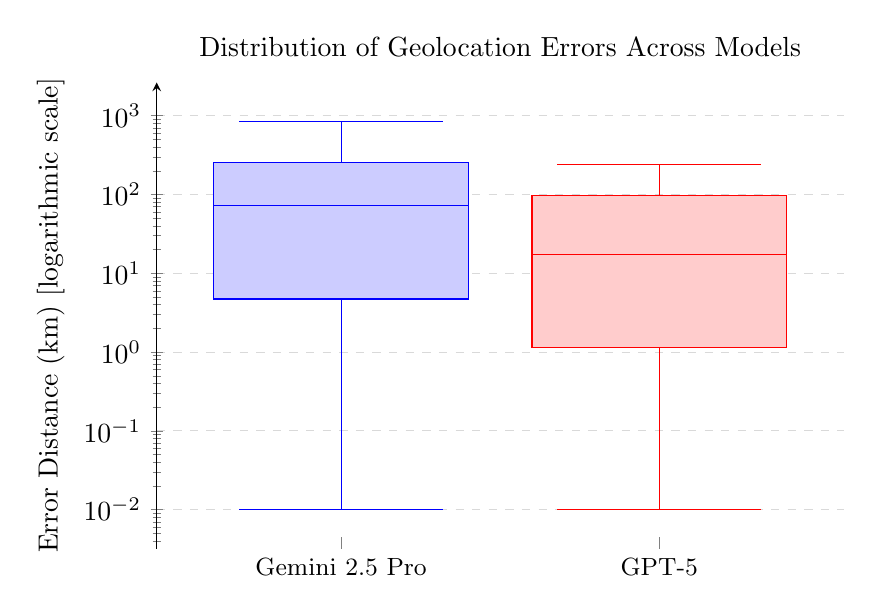
\begin{tikzpicture}
  \usepgfplotslibrary{statistics}
  \begin{axis}[
    title={Distribution of Geolocation Errors Across Models},
    boxplot/draw direction=y,
    x axis line style={opacity=0},
    axis x line*=bottom,
    axis y line=left,
    enlarge y limits=0.1,
    ymode=log,
    ylabel={Error Distance (km) [logarithmic scale]},
    xtick={1,2},
    xticklabels={Gemini 2.5 Pro, GPT-5},
    xticklabel style={font=\small},
    width=0.85\textwidth,
    height=7.5cm,
    ymajorgrids=true,
    grid style={dashed,gray!30},
  ]
  \addplot+ [
    boxplot prepared={
      median=73.31,
      upper quartile=252.25,
      lower quartile=4.72,
      upper whisker=850,
      lower whisker=0.01
    },
    color=blue,
    fill=blue!20,
  ] coordinates {};
  \addplot+ [
    boxplot prepared={
      median=17.53,
      upper quartile=97.75,
      lower quartile=1.15,
      upper whisker=240,
      lower whisker=0.01
    },
    color=red,
    fill=red!20,
  ] coordinates {};
  \end{axis}
  \end{tikzpicture}
  \caption{Error distribution comparison. GPT-5: median 17.53 km, IQR 96.60 km. Gemini 2.5 Pro: median 73.31 km, IQR 247.53 km.}
  \label{fig:boxplot}
\end{figure}

Cumulative distribution analysis (Figure~\ref{fig:cdf}) reveals GPT-5 achieves 100\% accuracy within 250 km, while Gemini 2.5 Pro reaches only 70\%.

\begin{figure}[H]
  \centering
  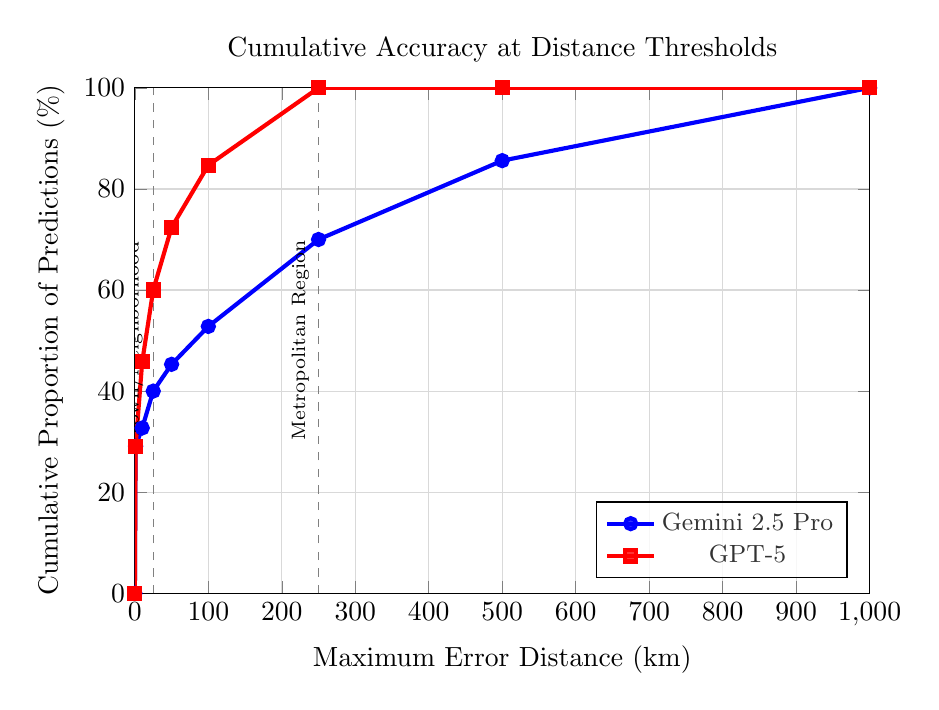
\begin{tikzpicture}
    \begin{axis}[
        title={Cumulative Accuracy at Distance Thresholds},
        xlabel={Maximum Error Distance (km)},
        ylabel={Cumulative Proportion of Predictions (\%)},
        xmin=0, xmax=1000,
        ymin=0, ymax=100,
        grid=both,
        major grid style={gray!30},
        minor grid style={gray!10},
        legend pos=south east,
        legend style={font=\small, fill=white, fill opacity=0.8, draw=black},
        width=0.9\textwidth,
        height=8cm,
        mark size=2pt,
    ]
    \addplot[mark=*, color=blue, thick, line width=1.5pt] coordinates { 
      (0, 0) (1, 29.1) (10, 32.7) (25, 40.0) (50, 45.3) (100, 52.8) (250, 70.0) (500, 85.6) (1000, 100.0) 
    };
    \addlegendentry{Gemini 2.5 Pro}
    \addplot[mark=square*, color=red, thick, line width=1.5pt] coordinates { 
      (0, 0) (1, 29.1) (10, 45.8) (25, 60.0) (50, 72.4) (100, 84.7) (250, 100.0) (500, 100.0) (1000, 100.0) 
    };
    \addlegendentry{GPT-5}
    
    % Add reference lines for key thresholds
    \draw[dashed, gray] (axis cs:25,0) -- (axis cs:25,100);
    \draw[dashed, gray] (axis cs:250,0) -- (axis cs:250,100);
    \node[anchor=south, font=\scriptsize, rotate=90] at (axis cs:25,50) {Town/Neighborhood};
    \node[anchor=south, font=\scriptsize, rotate=90] at (axis cs:250,50) {Metropolitan Region};
    \end{axis}
  \end{tikzpicture}
  \caption{Cumulative accuracy at distance thresholds. GPT-5 demonstrates superior performance below 250 km.}
  \label{fig:cdf}
\end{figure}

At 25 km, GPT-5 achieves 60\% accuracy vs. Gemini's 40\%. At 250 km, GPT-5 reaches 100\% while Gemini achieves 70\%. GPT-5 exhibits zero predictions in the 250--1000 km range. Figure~\ref{fig:buckets} shows the categorical distribution.

\begin{figure}[H]
  \centering
  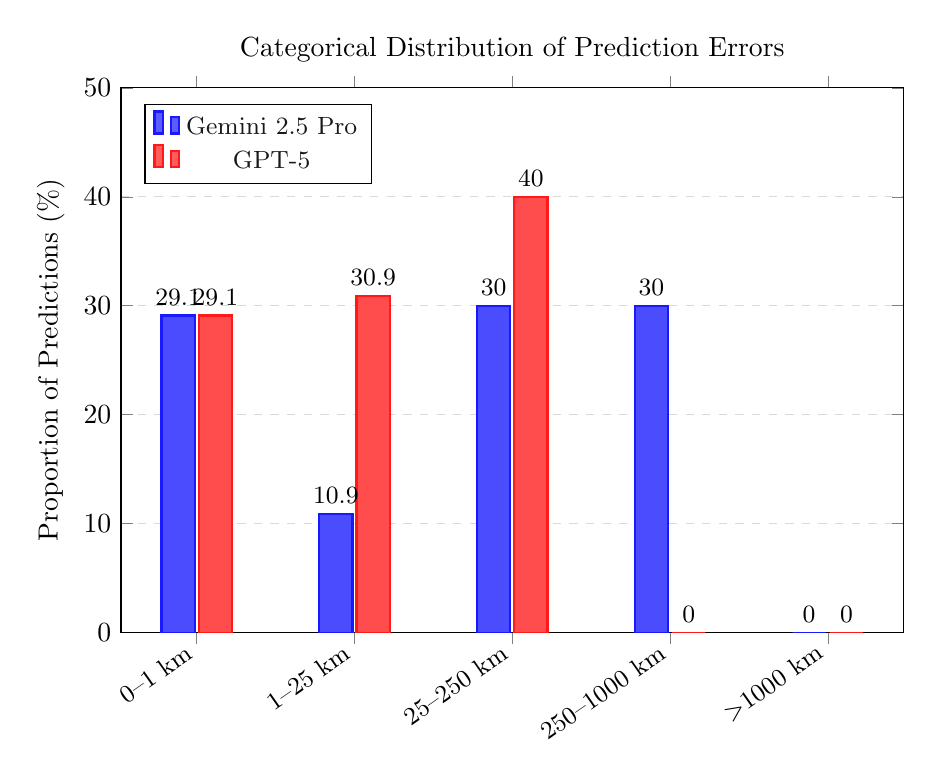
\begin{tikzpicture}
    \begin{axis}[
        ybar=1.5pt,
        bar width=12pt,
        title={Categorical Distribution of Prediction Errors},
        ylabel={Proportion of Predictions (\%)},
        symbolic x coords={0--1 km, 1--25 km, 25--250 km, 250--1000 km, ${>}$1000 km},
        xtick=data,
        xticklabel style={rotate=35, anchor=east, font=\small},
        nodes near coords,
        nodes near coords align={vertical},
        every node near coord/.append style={font=\small},
        legend pos=north west,
        legend style={font=\small, fill=white, fill opacity=0.9},
        ymin=0,
        ymax=50,
        ymajorgrids=true,
        grid style={dashed,gray!30},
        enlarge x limits=0.12,
        width=0.95\textwidth,
        height=8.5cm,
    ]
    \addplot[fill=blue!70, draw=blue!90, thick] coordinates {
      (0--1 km, 29.1) 
      (1--25 km, 10.9) 
      (25--250 km, 30.0) 
      (250--1000 km, 30.0) 
      (${>}$1000 km, 0.0)
    };
    \addplot[fill=red!70, draw=red!90, thick] coordinates {
      (0--1 km, 29.1) 
      (1--25 km, 30.9) 
      (25--250 km, 40.0) 
      (250--1000 km, 0.0) 
      (${>}$1000 km, 0.0)
    };
    \legend{Gemini 2.5 Pro, GPT-5}
    \end{axis}
  \end{tikzpicture}
  \caption{Bucket-wise error distribution. GPT-5 shows bounded error pattern (0\% in 250--1000 km range), while Gemini distributes 30\% in this bucket.}
  \label{fig:buckets}
\end{figure}

\begin{figure}[H]
  \centering
  \includegraphics[width=0.8\textwidth]{example_map.png}
  \caption{Visualization of a prediction error by Gemini 2.5 Pro. The actual location (53°36'19"N 1°57'29"W) and the predicted location (53°46'00.4"N 2°02'26.9"W) are separated by approximately 18.8 km. This illustrates the model's ability to identify the correct region while missing the precise street-level coordinates.}
  \label{fig:example_map}
\end{figure}

\begin{figure}[H]
  \centering
  \includegraphics[width=0.8\textwidth]{example_street_view.jpeg}
  \caption{The input image corresponding to the prediction in Figure~\ref{fig:example_map}. Sourced from a community-curated dataset, this image represents a non-standard perspective (e.g., a specific landmark or off-road view) rather than a typical street view. The model correctly identified the general UK region based on contextual clues but failed to pinpoint the exact location, illustrating the challenge of non-street-view imagery.}
  \label{fig:example_street_view}
\end{figure}

GPT-5 concentrates 40\% in the 25--250 km range and 30.9\% in 1--25 km, exhibiting a bounded error pattern. Gemini distributes evenly: 30\% in 25--250 km and 30\% in 250--1000 km, showing higher variance. Table~\ref{tab:statistics} summarizes the statistical comparison.

\begin{table}[H]
\centering
\caption{Statistical summary of prediction errors across 2,600 images per model.}
\label{tab:statistics}
\begin{tabular}{lcc}
\hline
\textbf{Metric} & \textbf{Gemini 2.5 Pro} & \textbf{GPT-5} \\
\hline
Median Error (km) & 73.31 & 17.53 \\
Mean Error (km) & 225.65 & 57.97 \\
Standard Deviation (km) & 294.81 & 69.58 \\
Interquartile Range (km) & 247.53 & 96.60 \\
\% Within 25 km & 40.0 & 60.0 \\
\% Within 250 km & 70.0 & 100.0 \\
\% in 250--1000 km range & 30.0 & 0.0 \\
\hline
\end{tabular}
\end{table}

The 4.2:1 median error ratio and GPT-5's complete absence of predictions in the 250--1000 km range represent fundamental behavioral differences rather than marginal performance variation.

\clearpage
\section{Discussion}

GPT-5 also shows regional consistency: 100\% of predictions within 250 km ($\sigma$ = 69.58 km) with a bounded error pattern (0\% in the range between 250--700~km). Gemini has a larger standard deviation ($\sigma$ = 294.81 km) with 30\% between the 250--1000 km range. Both have similar performance in terms of street-level accuracy (29.1\%). Remarkably, neither model produced catastrophic errors exceeding 1000 km in our analysis, indicating a strong baseline of continental-level understanding. GPT-5 will be appropriate for applications with predictable spatial resolution (content moderation, geotagging), and we may accept Gemini’s variance in cases of human verification or confidence filter before use. Distributional characterization is as important as comparative results for deployment actions.

\section{Conclusion}

We show that two models of equivalent aggregate accuracy (Gemini 2.5 Pro and GPT-5) have errors with qualitatively different distributions. GPT-5 obtains 100\% rate at less than 250 km (median: 17.53 km) with a confined error pattern, while more dispersed data is found for Gemini (30\%, median: 73.31 km) for d between 250 and 1000 km. Both achieve 29.1\% street-level precision. Models should focus on alignment of error distribution with application requirements rather than some aggregate metrics. Our study is limited by extrapolating our tests from 2,600 real images, and only test against/compare two models. Future work should consider mechanistic interpretations of error patterns and generalization to other spatially-grounded tasks.

\bibliographystyle{plainnat}
\bibliography{references}

\end{document}
